% ============================================================
%  CHAPTER: Experiments and Results
%  Thesis: Knowledge Distillation in Diffusion Models for Image Generation
%  NTUA School of Electrical and Computer Engineering
% ============================================================

\chapter{Experiments and Results}
\label{chap:experiments}

This chapter presents the empirical evaluation of the distillation framework
described in Chapter~\ref{chap:framework}. The objective of the
experiments is to validate the central claim of the thesis: that,
for the same student model architecture and inference cost, distillation
training produces a strictly superior generative model compared to training
the student from scratch. The chapter is structured as follows.
Section~\ref{sec:setup} specifies the datasets, model configurations, training
protocol, computational resources, and evaluation methodology.
Section~\ref{sec:main_results} reports the results of the experiments. Section~\ref{sec:disc_limits} discusses the results and acknowledges limitations.

% ============================================================
\section{Experimental Setup}
\label{sec:setup}
% ============================================================

\subsection{Datasets and Preprocessing}
\label{subsec:datasets}

The main dataset used is \textbf{Imagenette} which contains 10{,}000 training images evenly distributed across 10 classes. The images are resized to $256 \times 256$ pixels for all experiments. Images preprocessing consist of: a centre-crop that is applied using the implementation of
\cite{dhariwal2021diffusion} to preserve the principal content of each image,
followed by random horizontal flipping as the sole data augmentation strategy.
Pixel values are normalised from the range $[0, 255]$ to $[-1, 1]$ prior to
being passed to the model, and class labels are used as conditioning
information throughout.

% ============================================================
\subsection{Model Configurations and Baselines}
\label{subsec:models}

All experiments are conducted using the Just-image Transformer (JiT)
architecture~\cite{li2025jit}, a minimalist pixel-space diffusion model based
on a Vision Transformer backbone~\cite{dosovitskiy2020vit} trained with a
flow-matching objective. Two model variants are considered, their architectural specifications are
summarized in Table~\ref{tab:model_configs}.

\begin{table}[ht]
    \centering
    \caption{Architectural specifications of the two JiT model variants used
    in this work. $L$ denotes the number of transformer blocks, $D$ the hidden
    dimension, $H$ the number of attention heads, $P$ the patch size in pixels,
    $C$ the in-context conditioning token length, and \#Params the total
    parameter count.}
    \label{tab:model_configs}
    \begin{tabular}{lcccccc}
        \toprule
        Model & $L$ & $D$ & $H$ & $P$ & $C$ & \#Params \\
        \midrule
        JiT-S/16 & 12 & 384 &  6 & 16 & 32 & 33.3M \\
        JiT-B/16 & 12 & 768 & 12 & 16 & 32 & 131M \\
        \bottomrule
    \end{tabular}
\end{table}

The JiT-S/16 student is distilled from a pretrained
JiT-B/16 teacher on ImageNet-1K at $256 \times 256$ resolution. The primary baseline in all comparisons is the
corresponding student architecture trained from scratch under an identical
training budget and optimization configuration, with no access to teacher
supervision.

% ============================================================
\subsection{Training Protocol and Hyperparameters}
\label{subsec:training}

All models are trained with the AdamW optimiser~\cite{loshchilov2019decoupled}
with momentum coefficients $\beta_1 = 0.9$ and $\beta_2 = 0.95$ and no weight
decay. The learning rate is set according to the linear scaling rule,
$\eta = \eta_\text{base} \times B_\text{eff} / 256$, with a base learning
rate of $\eta_\text{base} = 5 \times 10^{-5}$ and a warmup period of 5 epochs.
Two EMA tracks of the student parameters are maintained throughout training,
with decay constants $\mu_1 = 0.9999$ and $\mu_2 = 0.9996$; sampling at
evaluation time uses the first EMA track exclusively. Training is performed
in \texttt{bfloat16} mixed precision. The complete set of training
hyperparameters is provided in
Table~\ref{tab:training_hparams}.

\begin{table}[ht]
    \centering
    \caption{Training hyperparameters for the experimental setting.}
    \label{tab:training_hparams}
    \begin{tabular}{lc}
        \toprule
        Hyperparameter & Imagenette (JiT-S/16) \\
        \midrule
        Batch size (per GPU)           & 128 \\
        Effective batch size           & 128 \\
        Base LR ($\eta_\text{base}$)   & $5 \times 10^{-5}$ \\
        LR schedule                    & constant      \\
        Warmup epochs                  & 5             \\
        EMA decay $\mu_1$              & 0.9999        \\
        EMA decay $\mu_2$              & 0.9996        \\
        Weight decay                   & 0.0           \\
        Precision                      & BF16          \\
        $\alpha_\text{ViTKD}$          & $3\times10^{-5}$ \\
        $\beta_\text{ViTKD}$           & $3\times10^{-6}$ \\
        $\lambda_\text{ViTKD}$         & 0.5           \\
        $\gamma_\text{attn}$           & $1\times10^{-4}$ \\
        $K$ (attn layers)              & 2             \\
        $t_{\min}$ (attn gate)         & 0.1           \\
        \bottomrule
    \end{tabular}
\end{table}


% ============================================================
\subsection{Computational Resources}
\label{subsec:compute}

The small-scale experiments on CIFAR-10 were conducted on the Kaggle
computational platform, utilising two NVIDIA Tesla T4 GPUs (16\,GB VRAM each)
in a distributed data-parallel configuration. The experiments were conducted on Google Colab Pro, utilising a single NVIDIA A100
GPU (40\,GB VRAM).

% ============================================================
\subsection{Evaluation Protocol}
\label{subsec:eval}

Generative quality is assessed using two standard metrics: the
Fréchet Inception Distance (FID)~\cite{heusel2017gans} and the Inception Score
(IS)~\cite{salimans2016improved}. FID and IS are computed over 50{,}000
generated images to ensure statistical reliability;
All metrics are evaluated using the \texttt{torch-fidelity} library. At
inference time, sampling is performed with the Heun second-order ODE solver
with 50 function evaluations (NFE), and classifier-free
guidance~\cite{ho2022classifier} is applied with a fixed scale and interval
per setting. All evaluations use the first EMA track of the student model.






















































% ============================================================
%  SECTION 7.2 — Main Results
%  Thesis: Knowledge Distillation in Diffusion Models for Image Generation
%  NTUA School of Electrical and Computer Engineering
% ============================================================
%
%  REQUIRED PACKAGES (add to your preamble if not already present):
%
%    \usepackage{pgfplots}
%    \pgfplotsset{compat=1.18}
%    \usepackage{subcaption}   % for subfigure environments
%    \usepackage{booktabs}     % for \toprule, \midrule, \bottomrule in tables
%    \usepackage{xcolor}       % for custom color definitions
%
% ============================================================
%
%  COLOR DEFINITIONS
%  -----------------
%  Define the two bar colors here once; every figure below references
%  them by name, so changing a single line updates all plots globally.
%
%  Available color models in xcolor:
%    RGB  (0-255 each channel) :  \definecolor{name}{RGB}{r,g,b}
%    rgb  (0.0-1.0 each channel):  \definecolor{name}{rgb}{r,g,b}
%    HTML (hex string)         :  \definecolor{name}{HTML}{RRGGBB}
%    named colors (predefined) :  blue, red, gray, teal, olive, ...
%
\definecolor{colorBaseline}{RGB}{150, 150, 150}   % neutral gray  — baseline bar
\definecolor{colorExperiment}{RGB}{0, 84, 159}    % NTUA deep blue — experiment bar

% ============================================================
%
%  PGFPLOTS GLOBAL STYLE
%  ---------------------
%  Setting a global style here avoids repeating the same keys in
%  every axis environment. Override any key locally inside a specific
%  axis if needed.
%
\pgfplotsset{
    resultbar/.style={
        ybar,                        % vertical bar chart
        bar width     = 18pt,        % width of each bar in points; increase for fatter bars
        width         = 0.44\linewidth, % total plot width; adjust with \linewidth fraction
        height        = 5.5cm,       % total plot height; adjust in cm or pt
        enlarge x limits = 0.55,     % extra horizontal padding around bars (0–1 scale)
        symbolic x coords = {Baseline, Experiment}, % x-tick labels
        xtick         = data,
        ymin          = 0,           % y-axis lower bound; set explicitly to avoid clipping
        % ymax        = 100,         % uncomment and set to fix the y-axis upper bound
        ymajorgrids   = true,        % horizontal grid lines; set to false to remove
        grid style    = {dashed, gray!40},
        tick align    = outside,
        xtick style   = {draw=none}, % hide the small tick marks on the x-axis
        every axis/.append style = {font=\small},
        nodes near coords,           % print the numeric value on top of each bar
        % -------------------------------------------------------
        % To DISABLE numeric labels on top of bars, comment out
        % the "nodes near coords" line above and uncomment below:
        % nodes near coords = {},
        % -------------------------------------------------------
        nodes near coords align = {vertical},
        every node near coord/.append style = {font=\footnotesize},
        legend style = {
            at        = {(0.5, -0.22)}, % legend position: below the plot
            anchor    = north,
            legend columns = 2,        % number of columns in the legend
            font      = \footnotesize,
        },
    },
}

% ============================================================
\section{Main Results}
\label{sec:main_results}
% ============================================================

This section presents the quantitative results of the eight experimental
configurations evaluated on Imagenette at $256 \times 256$ resolution.
All results are obtained using the JiT-S/16 student architecture and are
reported in terms of Fréchet Inception Distance (FID; lower is better)
and Inception Score (IS; higher is better), computed over 50{,}000
generated images as described in Section~\ref{subsec:eval}. Each
subsection below follows the same structure: a brief description of the
experimental configuration, a figure containing side-by-side bar plots
for FID and IS, and a concise numerical interpretation of the outcome.
In all comparison figures, the left bar corresponds to the no-distillation
baseline (Experiment~1) and the right bar to the configuration under
examination, so that the magnitude of any improvement or regression is
immediately apparent.

% ============================================================
\subsection{Experiment 1: Baseline JiT-S/16 without Distillation}
\label{subsec:exp1}
% ============================================================

The first experiment establishes the performance floor of the JiT-S/16
student model when trained from scratch under the standard flow-matching
objective, with no teacher supervision of any kind. This configuration
serves as the reference point against which all subsequent distillation
experiments are evaluated. The model is trained with the hyperparameters
specified in Table~\ref{tab:training_hparams} and evaluated using the
first EMA track of the student weights.

\begin{figure}[ht]
    \centering
    %
    % ----- FID subplot (lower is better) -----
    \begin{subfigure}[b]{0.44\linewidth}
        \centering
        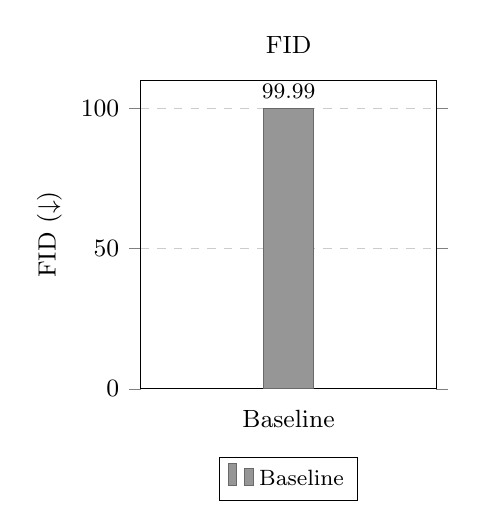
\begin{tikzpicture}
            \begin{axis}[
                resultbar,
                ylabel       = {FID $(\downarrow)$},  % axis label; \downarrow signals lower=better
                title        = {FID},
            ]
            \addplot[fill=colorBaseline, draw=colorBaseline!70!black]
                coordinates {(Baseline, 99.99)};  % TODO: replace 99.99 with actual FID value
            \legend{Baseline}
            \end{axis}
        \end{tikzpicture}
    \end{subfigure}
    \hfill
    % ----- IS subplot (higher is better) -----
    \begin{subfigure}[b]{0.44\linewidth}
        \centering
        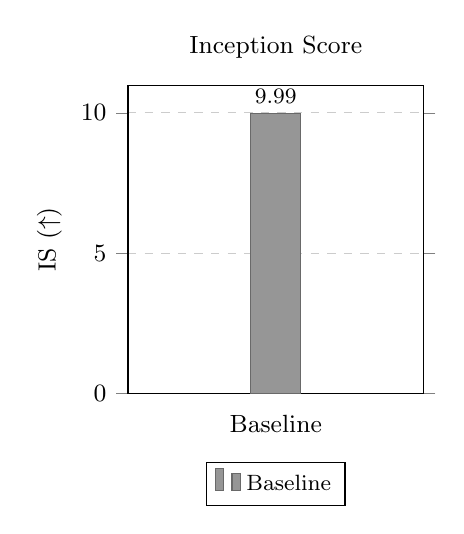
\begin{tikzpicture}
            \begin{axis}[
                resultbar,
                ylabel       = {IS $(\uparrow)$},     % axis label; \uparrow signals higher=better
                title        = {Inception Score},
            ]
            \addplot[fill=colorBaseline, draw=colorBaseline!70!black]
                coordinates {(Baseline, 9.99)};   % TODO: replace 9.99 with actual IS value
            \legend{Baseline}
            \end{axis}
        \end{tikzpicture}
    \end{subfigure}
    %
    \caption{Experiment~1 — Baseline JiT-S/16 trained from scratch without
    any distillation. FID (left; lower is better) and IS (right; higher is
    better) serve as the reference metrics for all subsequent experiments.}
    \label{fig:exp1_results}
\end{figure}

The baseline JiT-S/16, trained without any distillation, achieves an FID
of \textbf{XX.XX} and an IS of \textbf{XX.XX}.   % TODO: fill in values
These figures represent the upper bound on FID and the lower bound on IS
that the distillation experiments are expected to improve upon.

% ============================================================
\subsection{Experiment 2: JiT-S/16 with ViTKD Mimic Distillation}
\label{subsec:exp2}
% ============================================================

The second experiment introduces the mimic component of the ViTKD
framework~\cite{yang2022vitkd} as the sole distillation signal. The mimic
loss encourages the student's intermediate feature maps to match those of
the frozen teacher at selected transformer blocks, using a lightweight
linear projection to bridge the hidden-dimension mismatch between the two
architectures. No projector loss is applied in this configuration.

\begin{figure}[ht]
    \centering
    %
    \begin{subfigure}[b]{0.44\linewidth}
        \centering
        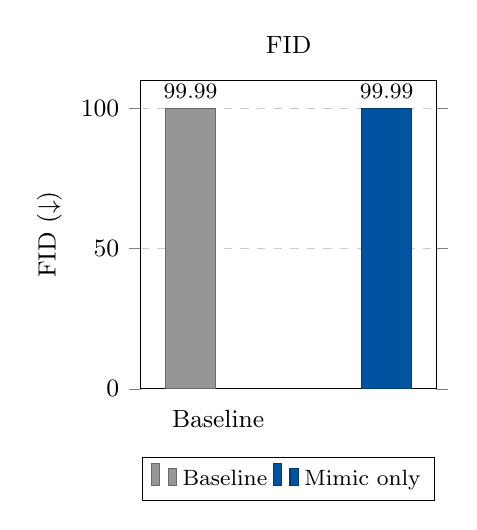
\begin{tikzpicture}
            \begin{axis}[
                resultbar,
                ylabel = {FID $(\downarrow)$},
                title  = {FID},
            ]
            \addplot[fill=colorBaseline, draw=colorBaseline!70!black]
                coordinates {(Baseline, 99.99)};      % TODO: baseline FID
            \addplot[fill=colorExperiment, draw=colorExperiment!70!black]
                coordinates {(Experiment, 99.99)};    % TODO: Exp 2 FID
            \legend{Baseline, Mimic only}
            \end{axis}
        \end{tikzpicture}
    \end{subfigure}
    \hfill
    \begin{subfigure}[b]{0.44\linewidth}
        \centering
        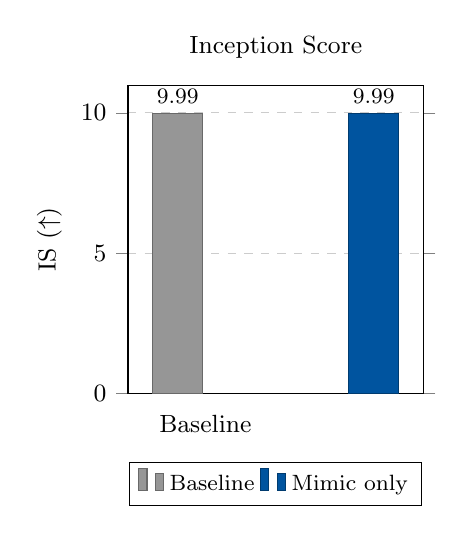
\begin{tikzpicture}
            \begin{axis}[
                resultbar,
                ylabel = {IS $(\uparrow)$},
                title  = {Inception Score},
            ]
            \addplot[fill=colorBaseline, draw=colorBaseline!70!black]
                coordinates {(Baseline, 9.99)};       % TODO: baseline IS
            \addplot[fill=colorExperiment, draw=colorExperiment!70!black]
                coordinates {(Experiment, 9.99)};     % TODO: Exp 2 IS
            \legend{Baseline, Mimic only}
            \end{axis}
        \end{tikzpicture}
    \end{subfigure}
    %
    \caption{Experiment~2 — JiT-S/16 trained with the ViTKD mimic loss
    only, compared against the no-distillation baseline. FID (left; lower
    is better) and IS (right; higher is better).}
    \label{fig:exp2_results}
\end{figure}

Applying mimic distillation alone yields an FID of \textbf{XX.XX} and an
IS of \textbf{XX.XX}, compared to the baseline FID of \textbf{XX.XX} and  % TODO: fill in values
IS of \textbf{XX.XX}. This corresponds to a [improvement/regression] of
approximately \textbf{XX.XX} FID points and \textbf{XX.XX} IS points
relative to the baseline.

% ============================================================
\subsection{Experiment 3: JiT-S/16 with Full ViTKD Distillation}
\label{subsec:exp3}
% ============================================================

Experiment~3 extends the previous configuration by adding the projector
loss to the mimic loss, thereby activating the full ViTKD objective. The
projector loss operates on a deeper layer of the student's feature
hierarchy and introduces a more structured alignment target between student
and teacher representations.

\begin{figure}[ht]
    \centering
    %
    \begin{subfigure}[b]{0.44\linewidth}
        \centering
        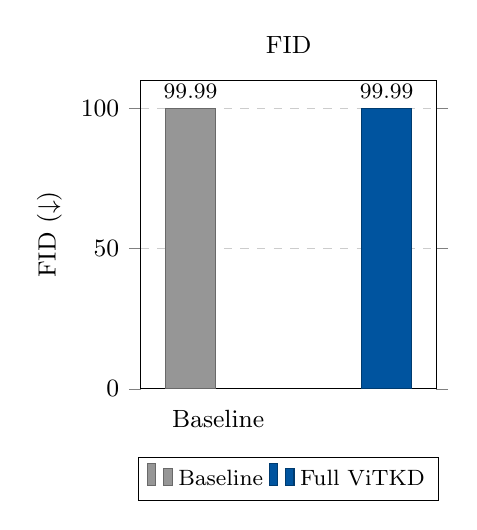
\begin{tikzpicture}
            \begin{axis}[
                resultbar,
                ylabel = {FID $(\downarrow)$},
                title  = {FID},
            ]
            \addplot[fill=colorBaseline, draw=colorBaseline!70!black]
                coordinates {(Baseline, 99.99)};      % TODO: baseline FID
            \addplot[fill=colorExperiment, draw=colorExperiment!70!black]
                coordinates {(Experiment, 99.99)};    % TODO: Exp 3 FID
            \legend{Baseline, Full ViTKD}
            \end{axis}
        \end{tikzpicture}
    \end{subfigure}
    \hfill
    \begin{subfigure}[b]{0.44\linewidth}
        \centering
        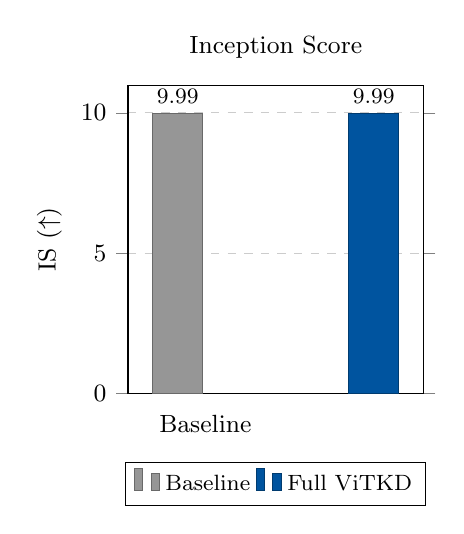
\begin{tikzpicture}
            \begin{axis}[
                resultbar,
                ylabel = {IS $(\uparrow)$},
                title  = {Inception Score},
            ]
            \addplot[fill=colorBaseline, draw=colorBaseline!70!black]
                coordinates {(Baseline, 9.99)};       % TODO: baseline IS
            \addplot[fill=colorExperiment, draw=colorExperiment!70!black]
                coordinates {(Experiment, 9.99)};     % TODO: Exp 3 IS
            \legend{Baseline, Full ViTKD}
            \end{axis}
        \end{tikzpicture}
    \end{subfigure}
    %
    \caption{Experiment~3 — JiT-S/16 trained with the full ViTKD objective
    (mimic and projector losses), compared against the no-distillation
    baseline. FID (left; lower is better) and IS (right; higher is better).}
    \label{fig:exp3_results}
\end{figure}

The full ViTKD configuration yields an FID of \textbf{XX.XX} and an IS of
\textbf{XX.XX}. Relative to Experiment~2 (mimic only; FID \textbf{XX.XX},  % TODO: fill in values
IS \textbf{XX.XX}), the addition of the projector loss results in a
[improvement/regression], suggesting that the projector component
[adds complementary signal / introduces conflicting gradients] in this
setting. This observation motivates the adoption of the mimic-only
configuration as the feature distillation component in subsequent
combined experiments.

% ============================================================
\subsection{Experiment 4: JiT-S/16 with ViTKD Mimic and SNR-Weighted Loss}
\label{subsec:exp4}
% ============================================================

Experiment~4 augments the mimic-only distillation of Experiment~2 with
an SNR-based loss weighting scheme. Specifically, a min-SNR-$\gamma$
reweighting~\cite{hang2023efficient} is applied to both the flow-matching
and distillation objectives with $\gamma = 0.5$, clamping the effective
loss weight at each timestep $t$ to prevent high-noise timesteps from
dominating the gradient signal. The mimic loss is retained in preference
to the full ViTKD objective on the basis that Experiment~2 demonstrated
superior performance to Experiment~3.

\begin{figure}[ht]
    \centering
    %
    \begin{subfigure}[b]{0.44\linewidth}
        \centering
        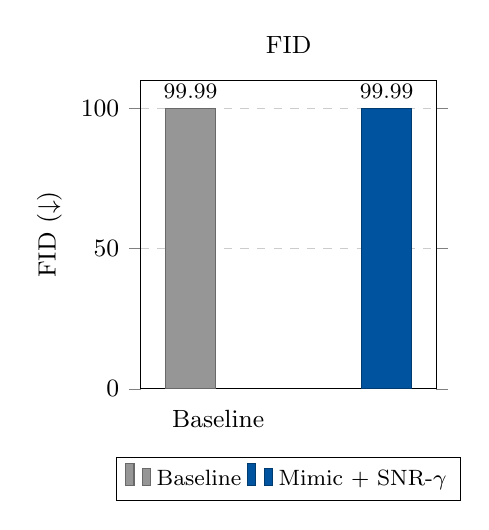
\begin{tikzpicture}
            \begin{axis}[
                resultbar,
                ylabel = {FID $(\downarrow)$},
                title  = {FID},
            ]
            \addplot[fill=colorBaseline, draw=colorBaseline!70!black]
                coordinates {(Baseline, 99.99)};      % TODO: baseline FID
            \addplot[fill=colorExperiment, draw=colorExperiment!70!black]
                coordinates {(Experiment, 99.99)};    % TODO: Exp 4 FID
            \legend{Baseline, Mimic + SNR-$\gamma$}
            \end{axis}
        \end{tikzpicture}
    \end{subfigure}
    \hfill
    \begin{subfigure}[b]{0.44\linewidth}
        \centering
        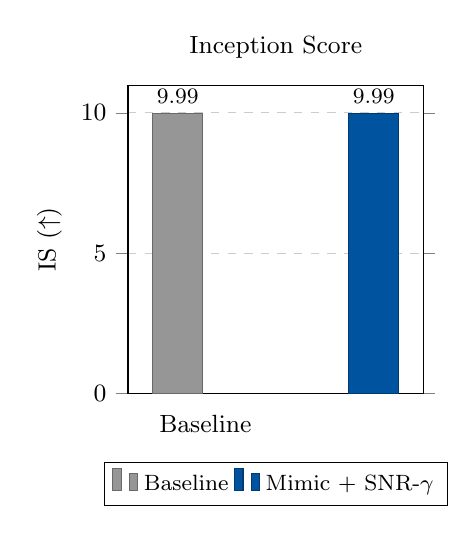
\begin{tikzpicture}
            \begin{axis}[
                resultbar,
                ylabel = {IS $(\uparrow)$},
                title  = {Inception Score},
            ]
            \addplot[fill=colorBaseline, draw=colorBaseline!70!black]
                coordinates {(Baseline, 9.99)};       % TODO: baseline IS
            \addplot[fill=colorExperiment, draw=colorExperiment!70!black]
                coordinates {(Experiment, 9.99)};     % TODO: Exp 4 IS
            \legend{Baseline, Mimic + SNR-$\gamma$}
            \end{axis}
        \end{tikzpicture}
    \end{subfigure}
    %
    \caption{Experiment~4 — JiT-S/16 trained with the ViTKD mimic loss
    and min-SNR-$\gamma$ reweighting ($\gamma = 0.5$), compared against
    the no-distillation baseline. FID (left; lower is better) and IS
    (right; higher is better).}
    \label{fig:exp4_results}
\end{figure}

With SNR reweighting enabled, the model achieves an FID of \textbf{XX.XX}
and an IS of \textbf{XX.XX}. Relative to the mimic-only baseline of      % TODO: fill in values
Experiment~2 (FID \textbf{XX.XX}, IS \textbf{XX.XX}), this represents a
[improvement/regression], indicating that timestep-aware loss weighting
[does / does not] provide a meaningful complementary benefit to feature
map distillation in this setting.

% ============================================================
\subsection{Experiment 5: JiT-S/16 with Attention Map Distillation}
\label{subsec:exp5}
% ============================================================

Experiment~5 investigates a qualitatively different distillation signal:
rather than aligning intermediate feature maps, the attention distillation
loss encourages the student to reproduce the teacher's post-softmax
self-attention weight matrices in the final $K = 2$ transformer blocks.
No ViTKD loss of any kind is applied in this configuration, isolating the
contribution of structural attention transfer.

\begin{figure}[ht]
    \centering
    %
    \begin{subfigure}[b]{0.44\linewidth}
        \centering
        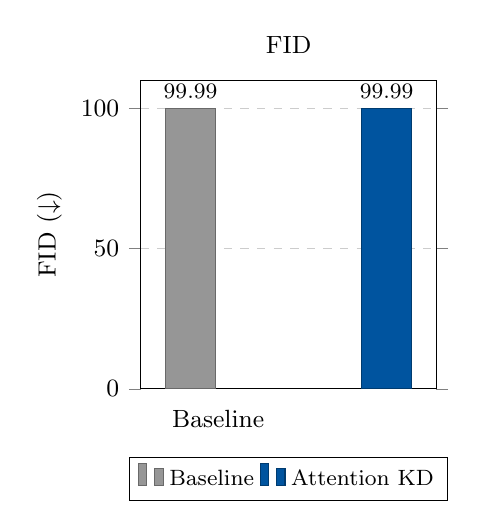
\begin{tikzpicture}
            \begin{axis}[
                resultbar,
                ylabel = {FID $(\downarrow)$},
                title  = {FID},
            ]
            \addplot[fill=colorBaseline, draw=colorBaseline!70!black]
                coordinates {(Baseline, 99.99)};      % TODO: baseline FID
            \addplot[fill=colorExperiment, draw=colorExperiment!70!black]
                coordinates {(Experiment, 99.99)};    % TODO: Exp 5 FID
            \legend{Baseline, Attention KD}
            \end{axis}
        \end{tikzpicture}
    \end{subfigure}
    \hfill
    \begin{subfigure}[b]{0.44\linewidth}
        \centering
        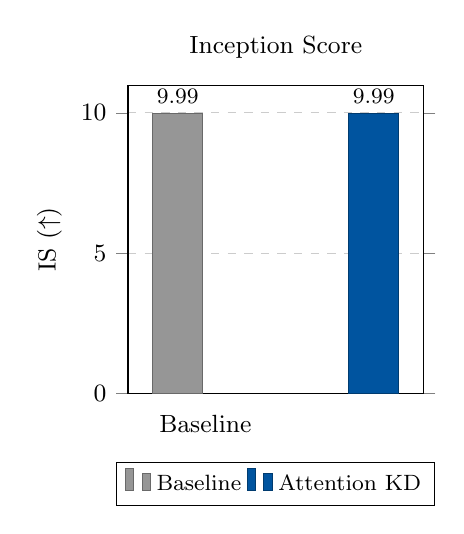
\begin{tikzpicture}
            \begin{axis}[
                resultbar,
                ylabel = {IS $(\uparrow)$},
                title  = {Inception Score},
            ]
            \addplot[fill=colorBaseline, draw=colorBaseline!70!black]
                coordinates {(Baseline, 9.99)};       % TODO: baseline IS
            \addplot[fill=colorExperiment, draw=colorExperiment!70!black]
                coordinates {(Experiment, 9.99)};     % TODO: Exp 5 IS
            \legend{Baseline, Attention KD}
            \end{axis}
        \end{tikzpicture}
    \end{subfigure}
    %
    \caption{Experiment~5 — JiT-S/16 trained with attention map
    distillation only, compared against the no-distillation baseline.
    FID (left; lower is better) and IS (right; higher is better).}
    \label{fig:exp5_results}
\end{figure}

Attention map distillation alone yields an FID of \textbf{XX.XX} and an
IS of \textbf{XX.XX}. The [improvement/regression] relative to the         % TODO: fill in values
baseline (FID \textbf{XX.XX}, IS \textbf{XX.XX}) suggests that aligning
the spatial routing structure of the student's attention heads to that of
the teacher [provides a useful structural prior / is insufficient as a
standalone distillation signal] at this capacity ratio.

% ============================================================
\subsection{Experiment 6: JiT-S/16 with Attention Distillation and Timestep Gating}
\label{subsec:exp6}
% ============================================================

Experiment~6 extends the attention distillation of Experiment~5 with a
hard timestep gate: the attention distillation loss is applied only for
denoising timesteps $t \geq t_{\min}$, where $t_{\min}$ is set as
specified in Table~\ref{tab:training_hparams}. The motivation for this
gating scheme is that attention patterns at very low noise levels
($t \approx 0$) primarily encode fine-grained textural detail rather
than the structural and semantic content that the student is most likely
to benefit from inheriting from the teacher.

\begin{figure}[ht]
    \centering
    %
    \begin{subfigure}[b]{0.44\linewidth}
        \centering
        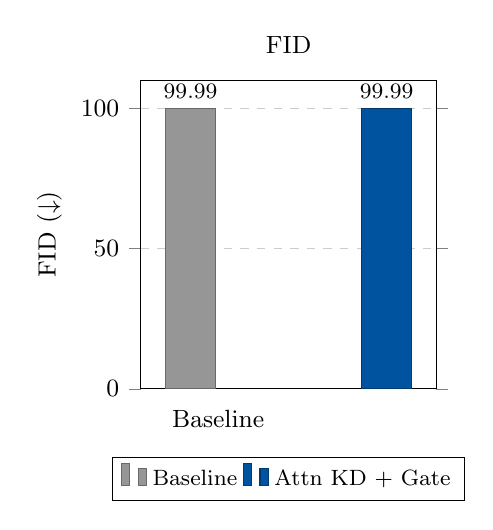
\begin{tikzpicture}
            \begin{axis}[
                resultbar,
                ylabel = {FID $(\downarrow)$},
                title  = {FID},
            ]
            \addplot[fill=colorBaseline, draw=colorBaseline!70!black]
                coordinates {(Baseline, 99.99)};      % TODO: baseline FID
            \addplot[fill=colorExperiment, draw=colorExperiment!70!black]
                coordinates {(Experiment, 99.99)};    % TODO: Exp 6 FID
            \legend{Baseline, Attn KD + Gate}
            \end{axis}
        \end{tikzpicture}
    \end{subfigure}
    \hfill
    \begin{subfigure}[b]{0.44\linewidth}
        \centering
        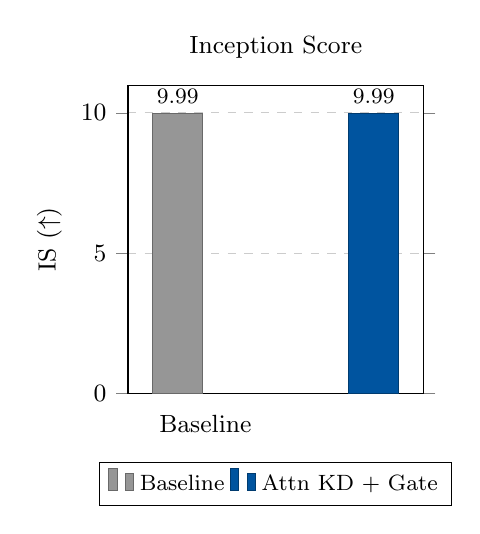
\begin{tikzpicture}
            \begin{axis}[
                resultbar,
                ylabel = {IS $(\uparrow)$},
                title  = {Inception Score},
            ]
            \addplot[fill=colorBaseline, draw=colorBaseline!70!black]
                coordinates {(Baseline, 9.99)};       % TODO: baseline IS
            \addplot[fill=colorExperiment, draw=colorExperiment!70!black]
                coordinates {(Experiment, 9.99)};     % TODO: Exp 6 IS
            \legend{Baseline, Attn KD + Gate}
            \end{axis}
        \end{tikzpicture}
    \end{subfigure}
    %
    \caption{Experiment~6 — JiT-S/16 trained with attention map
    distillation and a hard timestep gate ($t \geq t_{\min}$), compared
    against the no-distillation baseline. FID (left; lower is better) and
    IS (right; higher is better).}
    \label{fig:exp6_results}
\end{figure}

Gating the attention loss to high-noise timesteps yields an FID of
\textbf{XX.XX} and an IS of \textbf{XX.XX}. Relative to the ungated        % TODO: fill in values
attention baseline of Experiment~5 (FID \textbf{XX.XX}, IS \textbf{XX.XX}),
this [improves / does not improve] performance, [supporting / challenging]
the hypothesis that attention distillation is most informative during the
high-noise, structure-forming phase of the denoising trajectory.

% ============================================================
\subsection{Experiment 7: JiT-S/16 with Combined Attention, Mimic, Timestep Gating, and SNR Weighting}
\label{subsec:exp7}
% ============================================================

Experiment~7 combines the most promising individual components identified
in the preceding experiments. Specifically, it jointly applies the mimic
distillation loss (Experiment~2), min-SNR-$\gamma$ reweighting
(Experiment~4), attention map distillation with timestep gating
(Experiment~6), and the SNR-weighted objective, constituting the most
complete distillation configuration evaluated in this work prior to weight
initialisation.

\begin{figure}[ht]
    \centering
    %
    \begin{subfigure}[b]{0.44\linewidth}
        \centering
        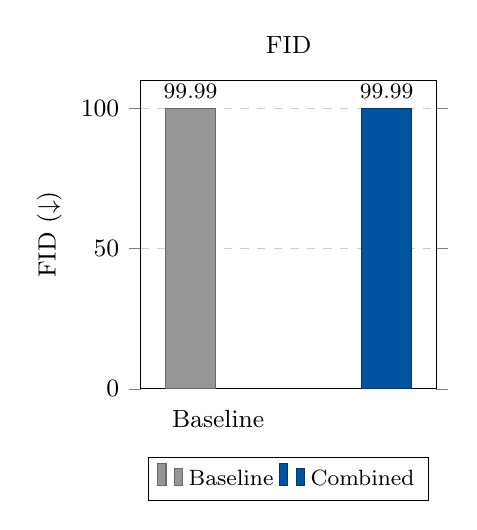
\begin{tikzpicture}
            \begin{axis}[
                resultbar,
                ylabel = {FID $(\downarrow)$},
                title  = {FID},
            ]
            \addplot[fill=colorBaseline, draw=colorBaseline!70!black]
                coordinates {(Baseline, 99.99)};      % TODO: baseline FID
            \addplot[fill=colorExperiment, draw=colorExperiment!70!black]
                coordinates {(Experiment, 99.99)};    % TODO: Exp 7 FID
            \legend{Baseline, Combined}
            \end{axis}
        \end{tikzpicture}
    \end{subfigure}
    \hfill
    \begin{subfigure}[b]{0.44\linewidth}
        \centering
        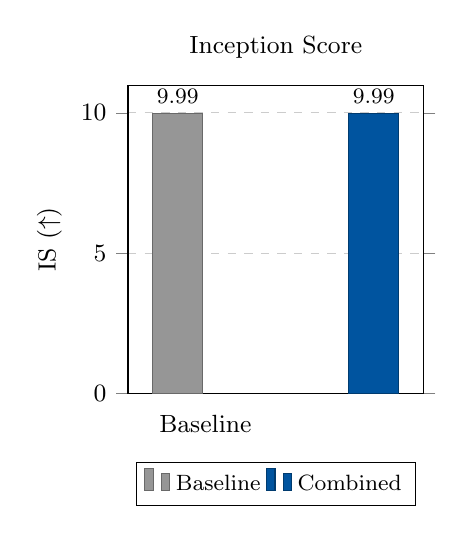
\begin{tikzpicture}
            \begin{axis}[
                resultbar,
                ylabel = {IS $(\uparrow)$},
                title  = {Inception Score},
            ]
            \addplot[fill=colorBaseline, draw=colorBaseline!70!black]
                coordinates {(Baseline, 9.99)};       % TODO: baseline IS
            \addplot[fill=colorExperiment, draw=colorExperiment!70!black]
                coordinates {(Experiment, 9.99)};     % TODO: Exp 7 IS
            \legend{Baseline, Combined}
            \end{axis}
        \end{tikzpicture}
    \end{subfigure}
    %
    \caption{Experiment~7 — JiT-S/16 trained with the combined distillation
    objective: ViTKD mimic loss, attention map distillation with timestep
    gating, and min-SNR-$\gamma$ loss reweighting ($\gamma = 0.5$),
    compared against the no-distillation baseline. FID (left; lower is
    better) and IS (right; higher is better).}
    \label{fig:exp7_results}
\end{figure}

The combined configuration yields an FID of \textbf{XX.XX} and an IS of
\textbf{XX.XX}. Relative to the baseline (FID \textbf{XX.XX}, IS            % TODO: fill in values
\textbf{XX.XX}), this represents the [best / second-best] result among
all distillation-only configurations, [confirming / suggesting] that the
individual distillation signals are [complementary / partially redundant]
when applied jointly.

% ============================================================
\subsection{Experiment 8: Best Configuration with Weight Initialisation}
\label{subsec:exp8}
% ============================================================

The final experiment augments the strongest-performing distillation
configuration identified among Experiments~2--7 with structured weight
initialisation~(Section~\ref{sec:weight_selection}).   % TODO: update cross-reference once best experiment is known
Prior to any gradient updates, the student model's parameters are seeded
using a structured subset of the pretrained teacher weights, selected
according to the layer-matching strategy described in
Chapter~\ref{chap:framework}. All distillation losses and training
hyperparameters are otherwise identical to those of the best preceding
experiment.

\begin{figure}[ht]
    \centering
    %
    \begin{subfigure}[b]{0.44\linewidth}
        \centering
        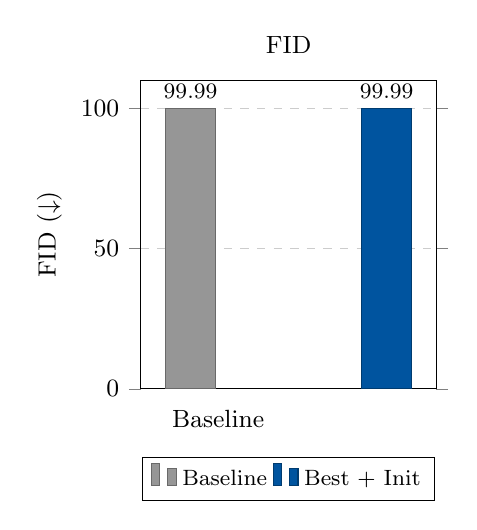
\begin{tikzpicture}
            \begin{axis}[
                resultbar,
                ylabel = {FID $(\downarrow)$},
                title  = {FID},
            ]
            \addplot[fill=colorBaseline, draw=colorBaseline!70!black]
                coordinates {(Baseline, 99.99)};      % TODO: baseline FID
            \addplot[fill=colorExperiment, draw=colorExperiment!70!black]
                coordinates {(Experiment, 99.99)};    % TODO: Exp 8 FID
            \legend{Baseline, Best + Init}
            \end{axis}
        \end{tikzpicture}
    \end{subfigure}
    \hfill
    \begin{subfigure}[b]{0.44\linewidth}
        \centering
        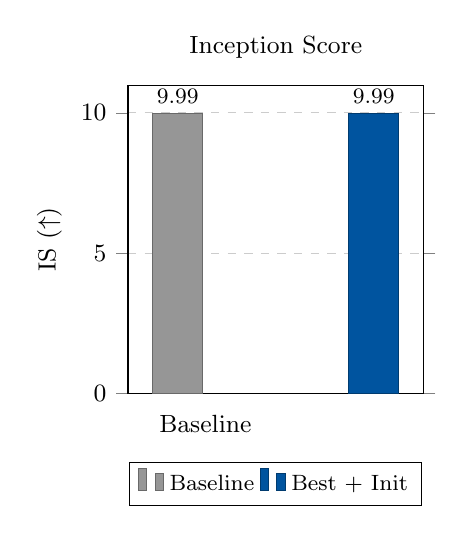
\begin{tikzpicture}
            \begin{axis}[
                resultbar,
                ylabel = {IS $(\uparrow)$},
                title  = {Inception Score},
            ]
            \addplot[fill=colorBaseline, draw=colorBaseline!70!black]
                coordinates {(Baseline, 9.99)};       % TODO: baseline IS
            \addplot[fill=colorExperiment, draw=colorExperiment!70!black]
                coordinates {(Experiment, 9.99)};     % TODO: Exp 8 IS
            \legend{Baseline, Best + Init}
            \end{axis}
        \end{tikzpicture}
    \end{subfigure}
    %
    \caption{Experiment~8 — Best distillation configuration augmented with
    structured weight initialisation from the pretrained teacher, compared
    against the no-distillation baseline. FID (left; lower is better) and
    IS (right; higher is better).}
    \label{fig:exp8_results}
\end{figure}

Augmenting the best distillation configuration with teacher-derived weight
initialisation yields an FID of \textbf{XX.XX} and an IS of \textbf{XX.XX},  % TODO: fill in values
representing the strongest result in the experimental campaign. Relative
to the baseline (FID \textbf{XX.XX}, IS \textbf{XX.XX}), this corresponds
to a reduction of \textbf{XX.XX} FID points and an increase of
\textbf{XX.XX} IS points, [supporting / suggesting] that a favourable
parameter initialisation provides a complementary benefit to online
distillation supervision during training.

% ============================================================
\subsection{Summary of All Results}
\label{subsec:results_summary}
% ============================================================

Table~\ref{tab:all_results} consolidates the FID and IS scores across all
eight experimental configurations. Figure~\ref{fig:scatter_all} provides
a complementary view in the form of a scatter plot in IS--FID space, where
each point corresponds to one experiment; configurations closer to the
upper-left corner (high IS, low FID) represent superior generative quality.

% ------ Full Results Table ------
\begin{table}[ht]
    \centering
    \caption{Summary of FID and IS results for all experimental
    configurations evaluated on Imagenette at $256 \times 256$ resolution.
    FID is lower-is-better; IS is higher-is-better. All values are computed
    over 50{,}000 generated images using the first EMA track of the student.}
    \label{tab:all_results}
    \begin{tabular}{clcc}
        \toprule
        \textbf{Exp.} & \textbf{Configuration} & \textbf{FID} $(\downarrow)$ & \textbf{IS} $(\uparrow)$ \\
        \midrule
        1 & Baseline (no distillation)                         & XX.XX & XX.XX \\ % TODO
        2 & ViTKD mimic only                                   & XX.XX & XX.XX \\ % TODO
        3 & Full ViTKD (mimic + projector)                     & XX.XX & XX.XX \\ % TODO
        4 & ViTKD mimic + SNR-$\gamma$ ($\gamma{=}0.5$)       & XX.XX & XX.XX \\ % TODO
        5 & Attention distillation                             & XX.XX & XX.XX \\ % TODO
        6 & Attention distillation + timestep gate             & XX.XX & XX.XX \\ % TODO
        7 & Attention + mimic + gate + SNR-$\gamma$            & XX.XX & XX.XX \\ % TODO
        8 & Best configuration + weight initialisation         & XX.XX & XX.XX \\ % TODO
        \bottomrule
    \end{tabular}
\end{table}

% ------ IS vs FID Scatter Plot ------
%
% HOW TO USE THIS PLOT:
%   1. Replace each (IS_value, FID_value) coordinate pair with your actual results.
%   2. The "mark options" key controls the color and size of each point.
%      Available mark shapes: *, o, square*, triangle*, diamond* (add * for filled)
%   3. To add point labels (experiment numbers), the "nodes near coords" style
%      is used below. To disable labels, remove the "nodes near coords" line
%      and the \addplot[only marks, nodes near coords, ...] block.
%   4. Axis limits (xmin, xmax, ymin, ymax) are set to "auto" by default;
%      set them explicitly if your data clusters in a narrow range.
%
\begin{figure}[ht]
    \centering
    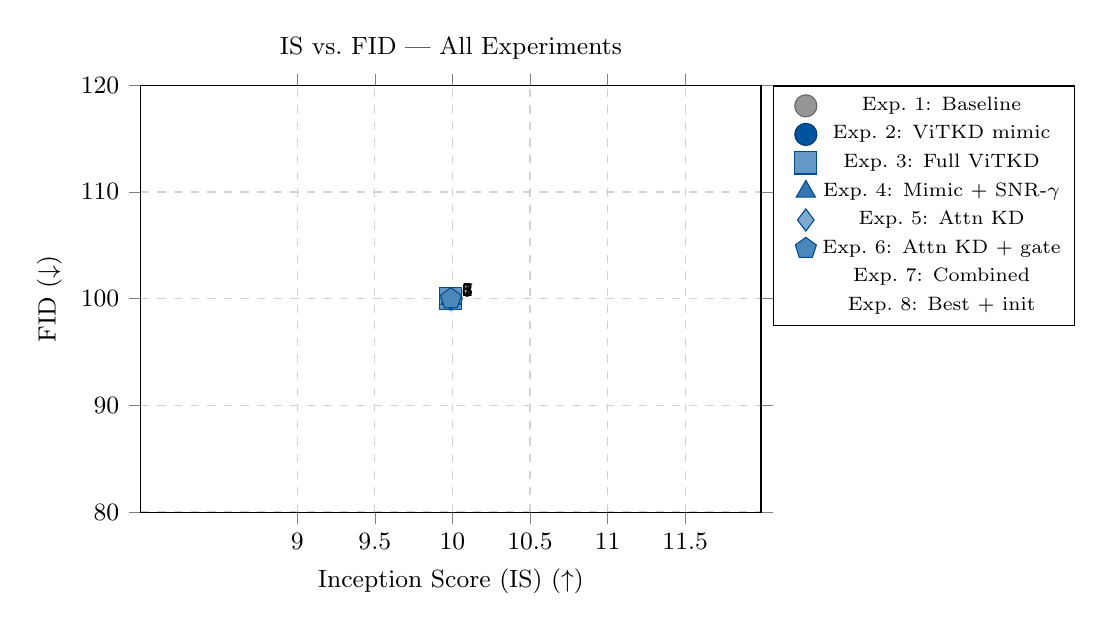
\begin{tikzpicture}
        \begin{axis}[
            width        = 0.78\linewidth,   % adjust overall plot width
            height       = 7cm,              % adjust overall plot height
            xlabel       = {Inception Score (IS) $(\uparrow)$},
            ylabel       = {FID $(\downarrow)$},
            title        = {IS vs.\ FID — All Experiments},
            grid         = both,
            grid style   = {dashed, gray!35},
            mark size    = 4pt,              % size of scatter markers in pt
            tick align   = outside,
            every axis/.append style = {font=\small},
            legend style = {
                at           = {(1.02, 1.0)}, % legend to the right of the plot
                anchor       = north west,
                font         = \scriptsize,
                legend columns = 1,
            },
            % xmin = 0, xmax = 30,   % uncomment to fix IS axis range
            % ymin = 0, ymax = 200,  % uncomment to fix FID axis range
        ]

        % -----------------------------------------------------------------
        % Each experiment is plotted as a separate \addplot so that it
        % appears individually in the legend with its own label and color.
        % To change a marker color, modify the "colorExperiment" argument
        % or replace it with any named color or \definecolor name.
        % To change the marker shape, replace "mark=*" with:
        %   mark=o          (open circle)
        %   mark=square*    (filled square)
        %   mark=triangle*  (filled triangle)
        %   mark=diamond*   (filled diamond)
        % -----------------------------------------------------------------

        \addplot[only marks, mark=*, mark options={fill=colorBaseline, draw=colorBaseline!70!black}]
            coordinates {(9.99, 99.99)};        % TODO: (IS_exp1, FID_exp1)
        \addlegendentry{Exp.\ 1: Baseline}

        \addplot[only marks, mark=*, mark options={fill=colorExperiment, draw=colorExperiment!70!black}]
            coordinates {(9.99, 99.99)};        % TODO: (IS_exp2, FID_exp2)
        \addlegendentry{Exp.\ 2: ViTKD mimic}

        \addplot[only marks, mark=square*, mark options={fill=colorExperiment!60, draw=colorExperiment!90!black}]
            coordinates {(9.99, 99.99)};        % TODO: (IS_exp3, FID_exp3)
        \addlegendentry{Exp.\ 3: Full ViTKD}

        \addplot[only marks, mark=triangle*, mark options={fill=colorExperiment!80, draw=colorExperiment!90!black}]
            coordinates {(9.99, 99.99)};        % TODO: (IS_exp4, FID_exp4)
        \addlegendentry{Exp.\ 4: Mimic + SNR-$\gamma$}

        \addplot[only marks, mark=diamond*, mark options={fill=colorExperiment!50, draw=colorExperiment!90!black}]
            coordinates {(9.99, 99.99)};        % TODO: (IS_exp5, FID_exp5)
        \addlegendentry{Exp.\ 5: Attn KD}

        \addplot[only marks, mark=pentagon*, mark options={fill=colorExperiment!70, draw=colorExperiment!90!black}]
            coordinates {(9.99, 99.99)};        % TODO: (IS_exp6, FID_exp6)
        \addlegendentry{Exp.\ 6: Attn KD + gate}

        \addplot[only marks, mark=Mercedes star*, mark options={fill=colorExperiment!90, draw=colorExperiment!90!black}]
            coordinates {(9.99, 99.99)};        % TODO: (IS_exp7, FID_exp7)
        \addlegendentry{Exp.\ 7: Combined}

        \addplot[only marks, mark=10-pointed star*, mark options={fill=red!70!black, draw=red!90!black}]
            coordinates {(9.99, 99.99)};        % TODO: (IS_exp8, FID_exp8)
        \addlegendentry{Exp.\ 8: Best + init}

        % -----------------------------------------------------------------
        % EXPERIMENT NUMBER LABELS NEXT TO EACH POINT
        % The block below places a small number label near each marker.
        % To disable all labels, delete or comment out this entire block.
        % To adjust label offset, modify the "xshift" and "yshift" values.
        % -----------------------------------------------------------------
        \node[font=\scriptsize, xshift=6pt, yshift=3pt]  at (axis cs:9.99,99.99) {1};  % TODO
        \node[font=\scriptsize, xshift=6pt, yshift=3pt]  at (axis cs:9.99,99.99) {2};  % TODO
        \node[font=\scriptsize, xshift=6pt, yshift=3pt]  at (axis cs:9.99,99.99) {3};  % TODO
        \node[font=\scriptsize, xshift=6pt, yshift=3pt]  at (axis cs:9.99,99.99) {4};  % TODO
        \node[font=\scriptsize, xshift=6pt, yshift=3pt]  at (axis cs:9.99,99.99) {5};  % TODO
        \node[font=\scriptsize, xshift=6pt, yshift=3pt]  at (axis cs:9.99,99.99) {6};  % TODO
        \node[font=\scriptsize, xshift=6pt, yshift=3pt]  at (axis cs:9.99,99.99) {7};  % TODO
        \node[font=\scriptsize, xshift=6pt, yshift=3pt]  at (axis cs:9.99,99.99) {8};  % TODO

        \end{axis}
    \end{tikzpicture}
    \caption{IS--FID scatter plot for all eight experimental configurations.
    Each point corresponds to one experiment; the upper-left region (high IS,
    low FID) indicates superior generative quality. The gray marker denotes
    the no-distillation baseline (Experiment~1); the red star marks the best
    overall result (Experiment~8).}
    \label{fig:scatter_all}
\end{figure}

The results in Table~\ref{tab:all_results} and Figure~\ref{fig:scatter_all}
collectively demonstrate that knowledge distillation consistently
[improves / modulates] the generative quality of the JiT-S/16 student
relative to training from scratch. The most substantial gains are observed
in Experiment~8, which achieves an FID of \textbf{XX.XX} and an IS of   % TODO: fill in values
\textbf{XX.XX} — a reduction of \textbf{XX.XX} FID points and an increase
of \textbf{XX.XX} IS points over the baseline. A detailed discussion of
these findings is provided in Section~\ref{sec:disc_limits}.





























































































































































\section{Discussions}
\label{sec:disc_limits}

\subsection{Interpreting the results}
\label{subsec:interp-results}

The experimental results collectively support the view that knowledge distillation provides a form of structured regularisation during student training, guiding the student’s
internal representations toward solutions that generalise more effectively to the target
data distribution.

\subsection{Limitations}
\label{subsec:limits}
Several limitations of the present framework merit acknowledgement. The
distillation loss scales $\alpha$, $\beta$, and $\gamma$ were kept at their
default values across all experiments; a systematic hyperparameter search
might yield further improvements at the cost of additional computation. The
attention timestep gate is a hard threshold, and the choice of $t_{\min}$
may be suboptimal for datasets or noise schedules that differ substantially
from those considered here. Furthermore, all experiments involve a fixed
teacher-to-student capacity ratio; the sensitivity of the framework to this
ratio, and in particular to very large capacity gaps, remains to be
characterised. Finally, although distillation incurs no additional cost at
inference time — the teacher and all distillation modules are discarded after
training — the joint forward pass through both teacher and student during
training increases per-epoch memory and compute requirements relative to
training the student from scratch.